\chapter{Map Data Sources}

\textcolor{orange}{NOE TEKST}

\section{Map Layers}

% KANKJE GLOSSARY FOR "COMPOSITE MAP"
The interactive map on the website supports multiple layers, allowing the user to build a composite map with various types of data. These layers include both meteorological and geological data relevant to assessing road conditions and the surrounding environment.

\subsection{Base Layers}

The user has the option to change the base layer of the map. In the current version, two options are available: the standard map from \Gls{openstreetmap}\footnote{\url{https://www.openstreetmap.org}} and the terrain map from OpenTopoMap\footnote{\url{https://opentopomap.org}}.
% KANSKJE GI GRUNN TIL HVORFOR DET IKKE KUN ER ETT BASE LAYER VALG

\begin{figure}[h]
     \centering
     \begin{subfigure}[b]{0.45\textwidth}
         \centering
         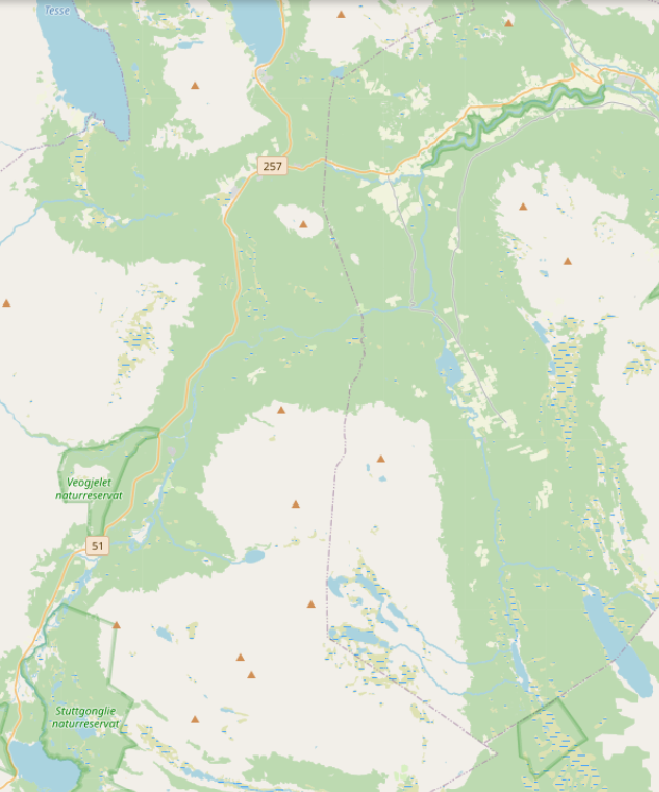
\includegraphics[width=\textwidth]{figures/base_layer_standard.pdf}
         \caption{Standard base layer}
         \label{fig:base_layer_standard}
     \end{subfigure}
     \hfill
     \begin{subfigure}[b]{0.45\textwidth}
         \centering
         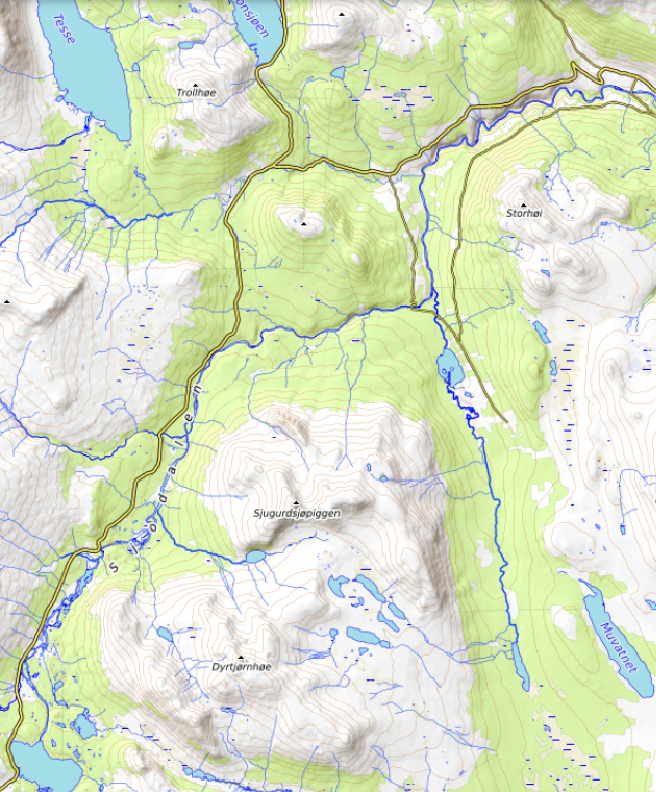
\includegraphics[width=\textwidth]{figures/base_layer_topo.pdf}
         \caption{Terrain base layer}
         \label{fig:base_layer_topo}
     \end{subfigure}
    \caption{Base map layer options}
    \label{fig:base_layers}
\end{figure}

\subsection{Superficial Deposits}
% LEGGE INN FARGE KODER FOR LØSMASSETYPE. TRENGER IKKE FOR ALLE? KANSKJE VEDLEGG?
The map layer showing superficial deposits is provided by \acrshort{ngu}. The superficial deposits data provide information on the distribution of surface sediments covering bedrock, mainly formed during and after the last Ice Age. It represents the dominant soil type in the upper layers, but does not account for deeper variations. These soil types include stones, gravel, sand, clay, peat, and moraine material \cite{geonorge_losmasser}. 

\begin{figure}[h]
    \centering
    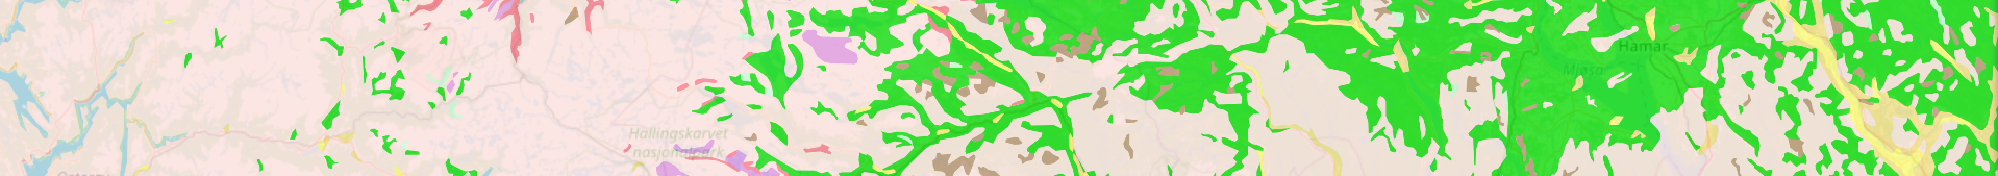
\includegraphics[width=1\linewidth]{figures/losmasse_eksempel.pdf}
    \caption{Example of the superficial deposits map layer}
    \label{fig:superficial_deposit_example}
\end{figure}

\subsection{Frost Depth}

% Kanskje nevn GWB modellen? https://www.senorge.no/WaterMap
% TODO: DOBBELSJEKK AT VI SKAL BRUKE 10CM FOR TELE
The frost depth map layer, provided by \acrshort{nve}, visualizes frost depth as a raster map, with colors ranging from dark blue (indicating deep frost) to light green (indicating no frost). This layer is particularly useful for assessing the trafficability of forestry roads. When frost depth reaches 10 cm or more (see \hyperref[tab:frost_depth_classification]{Table~\ref*{tab:frost_depth_classification}}), road conditions are generally suitable for heavy vehicles. As a result, most forestry roads tend to have good trafficability throughout the Norwegian winter, when frost is typically present.

% KANSKJE GI EKSEMPLER PÅ NÅR (OG HVOR) DET ER VANLIG MED DE FORSKJELLIGE DYBDENE
\begin{table}[h]
    \centering
    \begin{tabular}{|l|l|l|}
        \hline  
        \textbf{Color} & \textbf{Frost Depth} & \textbf{Depth in cm} \\
        \hline
        \cellcolor[HTML]{00009c} & Very Deep Frost & > 75 cm \\
        \hline
        \cellcolor[HTML]{0018ff} & Deep Frost & 30-75 cm \\
        \hline
        \cellcolor[HTML]{009aff} & Frost & 10-30 cm \\
        \hline
        \cellcolor[HTML]{84ebff} & Shallow Frost & 5-10 cm \\
        \hline
        \cellcolor[HTML]{deffff} & Partially Frost-free & 0-5 cm \\
        \hline
        \cellcolor[HTML]{cef77b} & No Frost & 0 cm \\
        \hline
    \end{tabular}
    \caption{Frost depth classification and corresponding colors \cite{nve2025waterdata}}
    \label{tab:frost_depth_classification}
\end{table}

\begin{figure}[h]
    \centering
    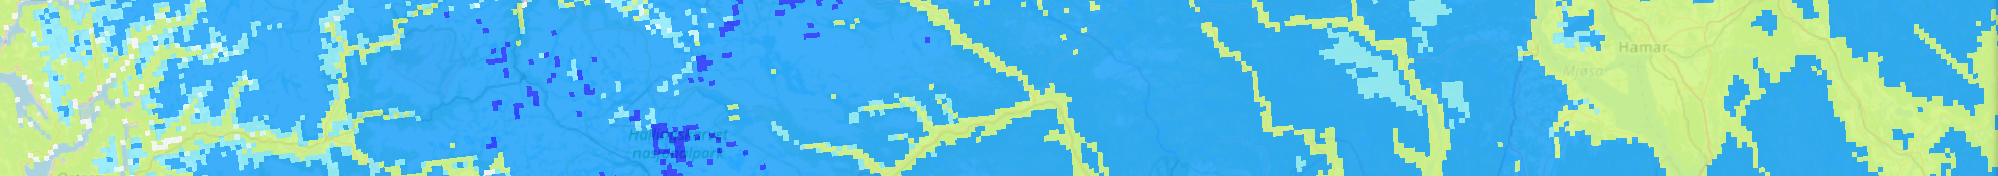
\includegraphics[width=1\linewidth]{figures/teledyp_eksempel.pdf}
    \caption{Example of the frost depth map layer}
    \label{fig:frost_depth_example}
\end{figure}

\subsection{Soil Saturation}

% Glossary groundwater & root zone
The soil saturation data, provided by NVE, represents the ratio between the current simulated water content in the groundwater and root zone and the highest value observed during the historical reference period from 1981 to 2010 \cite{nve2025waterdata}. For example, a soil saturation level of 70\% indicates that the soil currently holds 70\% of the maximum water content recorded during that period.

Soil saturation can be used to assess \gls{trafficability}, which refers to the highest level of soil moisture a road can tolerate without experiencing unacceptable deformation. This threshold varies depending on the type of superficial deposits present, as different materials have varying levels of permeability \cite{fjeld2023trafficability}.

\begin{table}[h]
    \centering
    \begin{tabular}{|l|l|}
        \hline  
        \textbf{Color} & \textbf{Soil Saturation (\%)} \\
        \hline
        \cellcolor[HTML]{f82200} & Above 90\% \\
        \hline
        \cellcolor[HTML]{f8c400} & 80 - 90\% \\
        \hline
        \cellcolor[HTML]{f8fc00} & 70 - 80\% \\
        \hline
        \cellcolor[HTML]{29d460} & 60 - 70\% \\
        \hline
        \cellcolor[HTML]{e4e4e4} & Under 60\% \\
        \hline
    \end{tabular}
    \caption{Soil saturation classification and corresponding colors \cite{nve2025waterdata}}
    \label{tab:soil_saturation_classification}
\end{table}

\subsection{Forestry Roads}

The forestry roads map layer is a vector dataset retrieved via a WFS service in GeoJSON format, provided by GeoNorge and Kartverket. In the GeoJSON, forestry roads are represented as geometric LineString features, where each LineString defines a segment between two coordinates. A single road is often divided into multiple such features. The GeoJSON also includes properties of each features such as road number, municipality number, and feature length.

\textcolor{orange}{Skrive om at implmenetation kommer senere, men nevne korte trekk hva layeret er.}

\section{Gridded Water Balance Model}

The Gridded Water Balance (GWB) model is responsible for calculating the hydrological variables shown in the SeNorge\footnote{\url{https://www.senorge.no}} grid maps. It is a spatially distributed adaptation of the HBV model, which was initially designed for flood forecasting, and it calculates water balance for each \qty{1}{\kilo\meter\squared} grid cell separately \cite{nve2025waterdata}.

Each grid cell is characterized by its average elevation and the distribution of land cover types, such as vegetation, soil, wetlands, lakes, and glaciers. The model operates on a daily time step, using spatially distributed data for temperature and precipitation as its inputs \cite{nve2025waterdata}.

GWB includes processes for snow storage, root zone moisture, groundwater storage, evaporation, runoff to rivers, wetlands, lakes, frost depth, and glaciers. Potential evaporation is calculated based on air temperature and vegetation development during the growing season, while actual evaporation is limited by the availability of soil moisture \cite{nve2025waterdata}.

Water balance calculations are conducted independently for each grid cell. The parameterization of each cell incorporates variations in topography, vegetation, and soil type, reflecting their impact on local hydrological processes \cite{nve2025waterdata}.

Both the frost depth and soil saturation map layers from SeNorge and NVE are derived using the GWB model.

\section{Sources of Uncertainty}

\textcolor{orange}{Gjerne skriv om feilkilder fra andre en senorge dataen}

Various factors contribute to uncertainties in the frost depth and soil saturation maps. These include possible errors in the interpolation of meteorological and soil data, as well as limitations in how the model translates real-world conditions. These uncertainties are especially important around the freezing point (0°C), where even minor temperature variations can influence whether precipitation falls as rain or snow, or if snow begins to melt \cite{senorge_watermap}. The frost depth map tends to provide more accurate simulations of soil freezing compared to soil thawing \cite{nve2025waterdata}.

Localized weather events, such as isolated rain showers missed by nearby weather stations, may also go unnoticed. Furthermore, environmental factors like wind, humidity, and solar radiation, which are not accounted for in the model, can speed up snowmelt, causing discrepancies between the model’s predictions and actual conditions \cite{senorge_watermap}.

The SeNorge maps show daily averages, which may miss short-term variations like intense rainfall or rapid changes in temperature within a single day. The forecast maps predict up to nine days ahead, with increasing uncertainty the further into the future the prediction extends. Finally, the model's representation of vegetation and soil types may not always be accurate, potentially leading to the overestimation or underestimation of soil saturation levels \cite{senorge_watermap}.